% ARPEGOS:  Automatized Roleplaying-game Profile Extensible Generator Ontology based System %
% Author : Alejandro Muñoz Del Álamo %
% Copyright 2019 %

% Section 3.4: Alternativas de Solución %

\section{Alternativas de Solución}
En esta sección, se ofrece un estudio del arte de las diferentes alternativas tecnológicas que permitan satisfacer 
los requerimientos del sistema, para optar por una de las opciones planteadas, que será dispuesta como base 
para el software a desarrollar.\medskip

Con este motivo, hemos optado por recoger algunas de las tecnologías existentes para realizar desarrollo de aplicaciones 
móviles.

\subsection{Android Studio}
Android Studio es el entorno de desarrollo integrado (\textit{IDE}) oficial para el desarrollo de apps para Android, 
basado en \textit{IntelliJ IDEA} de \textit{JetBrains} y ha sido publicado gratuitamente a través de la Licencia Apache 2.0.
Disponible para las plataformas \textit{Windows}, \textit{macOS} y \textit{GNU/Linux}. Basado en el lenguanje \textit{Java},
no tiene herramientas nativas para trabajar directamente con \textit{RDF} y \textit{OWL}. Para suplir este obstáculo, 
haríamos uso del framework libre \textit{Apache Jena}, cuya API permite trabajar con RDF, consiguiendo vincular 
el desarrollo en aplicaciones móviles con el uso de ontologías.

\begin{figure}[H]
    \centering
    \begin{minipage}{5cm}
        \centering
        
\includegraphics[width=5cm]{Images/Logo_Android_Studio.png}
        \caption{Logo de \textit{Android Studio}}  
    \end{minipage}
    \hfill
    \begin{minipage}{5cm}
        \centering
        
\includegraphics[width=5cm]{Images/Logo_Jena.png}
        \caption{Logo de \textit{Apache Jena}}  
    \end{minipage}
\end{figure}
% https://es.wikipedia.org/wiki/Android_Studio
% https://jena.apache.org/

\subsection{React Native}
React Native es un \textit{framework} para el desarrollo de aplicaciones móviles de código abierto desarrollado por 
\textit{Facebook}. Se utiliza para desarrollar aplicaciones para \textit{Android}, \textit{iOS}, \textit{Web} y 
\textit{UWP} permitiendo a los desarrolladores usar \textit{React} con funcionalidades nativas de las plataformas.
Al igual que \textit{Android Studio}, React Native no tiene herramientas nativas para el desarrollo de ontologías, de 
manera que haríamos uso de bibliotecas tales como \textit{rdflib.js} para poder proceder al tratamiento de las ontologías.

\begin{figure}[H]
    \centering
    \begin{minipage}{5cm}
        \centering
        
\includegraphics[width=5cm]{Images/Logo_React.jpeg}
        \caption{Logo de \textit{React Native}}  
    \end{minipage}
    \hfill
    \begin{minipage}{5cm}
        \centering
        
\includegraphics[width=5cm]{Images/Logo_Rdflib.jpeg}
        \caption{Logo de \textit{rdflib.js}}  
    \end{minipage}
\end{figure}
% https://en.wikipedia.org/wiki/React_Native
% https://github.com/linkeddata/rdflib.js

\subsection{Xamarin}
Xamarin es una plataforma de código abierto para compilar aplicaciones modernas y con mejor rendimiento para \textit{iOS}, 
\textit{Android} y \textit{Windows} con \textit{\dotnet}. Xamarin es una capa de abstracción que administra la comunicación 
de código compartido con el código de plataforma subyacente. Xamarin dispone de una biblioteca conocida como 
\textit{RDFSharp}, que permite generar y procesar ontologías en formatos \textit{RDF} y \textit{OWL}.

\begin{figure}[H]
    \centering
    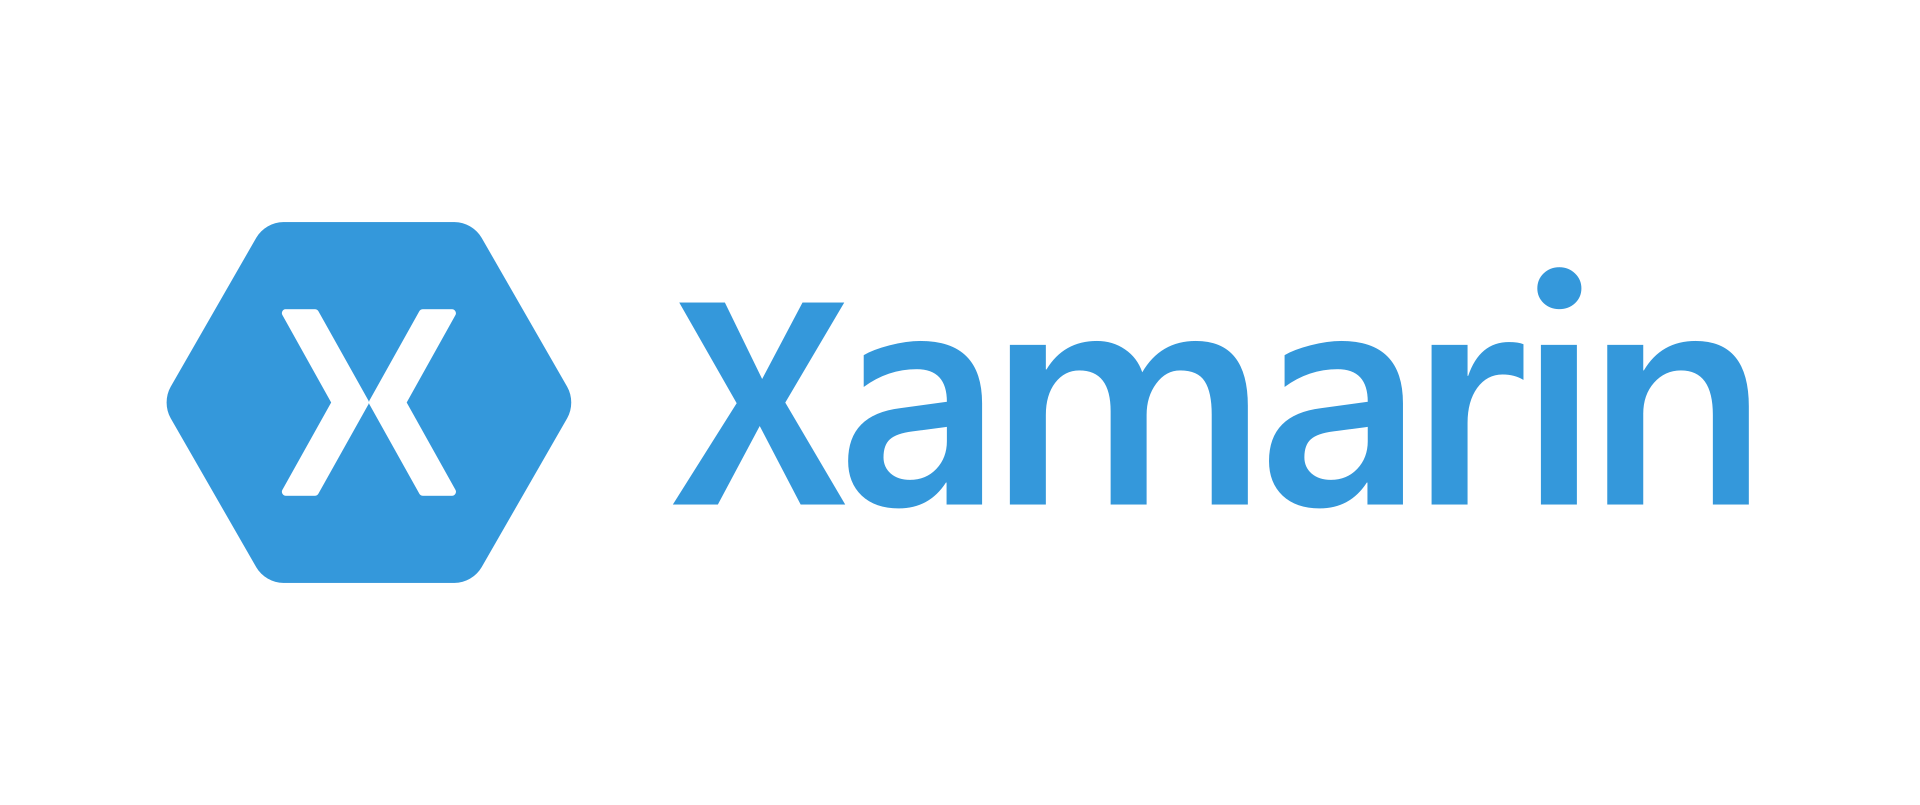
\includegraphics[width=5cm]{Images/Logo_Xamarin.png}
    \caption{Logo de \textit{Xamarin}}
\end{figure}
% https://docs.microsoft.com/es-es/xamarin/get-started/what-is-xamarin
% https://github.com/mdesalvo/RDFSharp
